%\subsection{Perturbation}
\subsection{Differential Privacy}\label{sec:dp}

Differential Privacy ist eine Technik, welche 2006 von Cynthia Dwork \cite{P-26} vorgestellt wurde.
Ziel dabei ist es, Zugriff auf einen Datensatz zu ermöglichen, der sowohl nützliche Erkenntnisse zulässt, als auch die Privatsphäre eines einzelnen Datenpunktes schützt.

Differential Privacy kann dabei an 3 unterschiedlichen Stellen der Machine Learning Pipeline genutzt werden:
\begin{compactitem}
\item \textbf{Vorbereitung der Trainingsdaten:} Diese Methodik wird folgend in diesem Kapitel erläutert.
\item \textbf{Trainingsalgorithmus:} Kapitel \ref{sec:dp_training} beschreibt, welche Anpassung am Trainingsalgorithmus vorgenommen werden müssen, damit dieser Differential Privacy nutzen kann.
\item \textbf{Vorhersage des Modells:} Wie der Output des Modells durch Nutzung von Differential Privacy geschützt werden kann, wird durch Kapitel \ref{sec:dp_output} dargestellt.
\end{compactitem}


Differential Privacy laut Dwork \cite{P-26} sorgt dafür, dass die gleiche Anfrage auf zwei unterschiedlichen Datensätze, die in höchstens einem Datenpunkt voneinander abweichen, keine signifikant unterschiedlichen Ergebnisse aufweise. 
Um dies zu erreichen, wird den Anfragen ein zufälliges Rauschen hinzugefügt. 
Dadurch handelt es sich bei Abfragen um randomisierte Funktionen.
Die Größe des Unterschied der gleichen Abfrage auf zwei Datensätze, die sich in höchstens einem Eintrag unterscheiden, kann durch einen Wert $\epsilon$ dargestellt werden.

Formal lautet die Definition von $\epsilon$-Differential Privacy wie folgt \cite{P-26}:\\
\textit{
Eine randomisierte Funktion $M$, welche einen Datensatz $D$ auf einen Wertebereich $R$ abbildet, weist $\epsilon$-Differential Privacy auf, wenn für alle Datensätze $D_{1}$ und $D_{2}$ die sich in höchstens einem Datenpunkt unterscheiden, gilt:}
\begin{equation}
    Pr[M(D_{1}) \in R] \leq e^{\epsilon} \times Pr[M(D_{2}) \in R]
\end{equation}

Dwork und Roth \cite{P-27} fügten der Definition noch einen Parameter $\delta$ hinzu, welcher erlaubt, dass die Voraussetzungen zu einem definierten Grad verletzt werden können.
Die damit angepasste Definition von ($\epsilon$,$\delta$)-Differential Privacy lautet \cite{P-27}:\\
%Damit lautet die formale Definition von Differential Privacy wie folgt \cite{P-27}:
\textit{
    Eine randomisierte Funktion $M$, welche einen Datensatz $D$ auf einen Wertebereich $R$ abbildet, erfüllt ($\epsilon$,$\delta$)-Differential Privacy, wenn für alle Datensätze $D_{1}$ und $D_{2}$, die sich in höchstens einem Datenpunkt unterscheiden, gilt:}
\begin{equation}
    Pr[M(D_{1}) \in R] \leq e^{\epsilon} \times Pr[M(D_{2}) \in R] + \delta
\end{equation} 

Konkret sagen die Definitionen aus, dass eine randomisierte Funktion, auf beiden Datensätzen angewendet, nahezu die gleichen Ergebnisse liefert. 
Dabei bestimmten $\epsilon$ und $\delta$ wie stark sich die Ergebnisse unterscheiden dürfen. 
Kleinere Werte bedeuten dabei, dass die Privatsphäre besser geschützt ist, was sich jedoch negativ auf die Nützlichkeit der Abfragen auswirkt.

\begin{figure}[!htb]
    \centering
    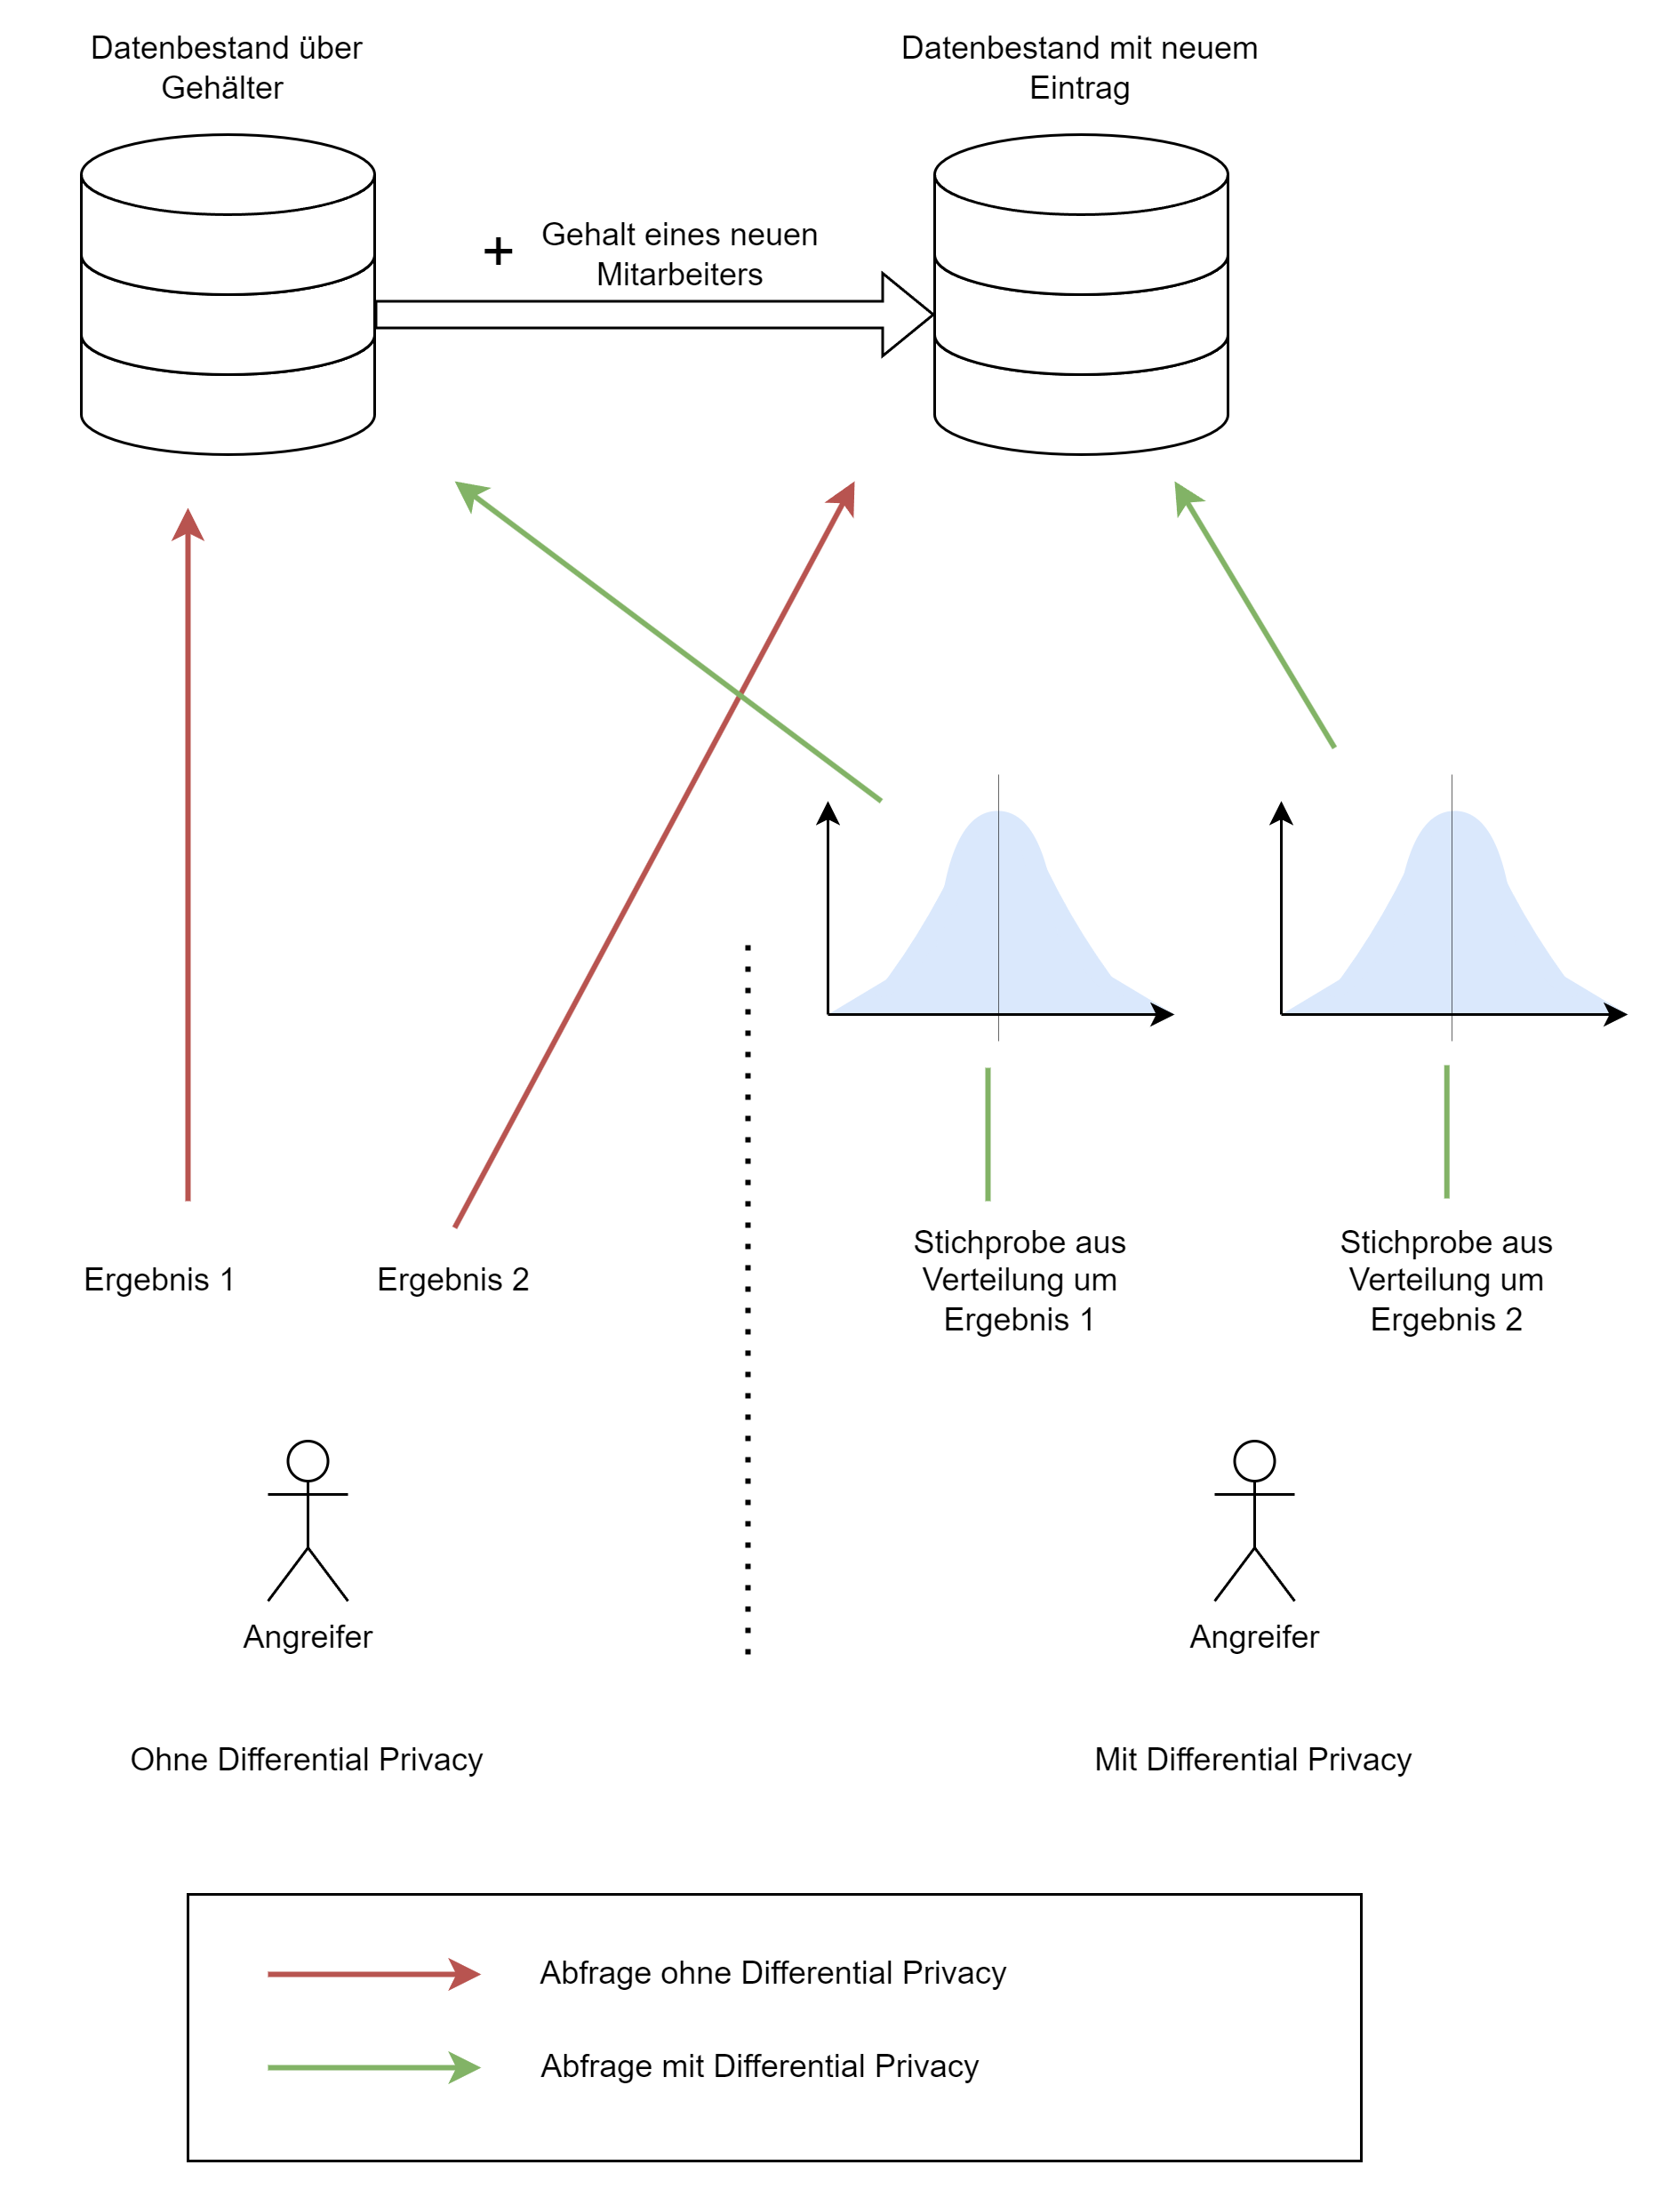
\includegraphics[width=10cm]{figures/dp}
    \caption{Beispiel Differential Privacy}
    \label{fig:dp}
\end{figure} 

Abbildung \ref{fig:dp} zeigt exemplarisch, wie Differential Privacy anhand einer Abfrage des Durchschnittsgehalts eines Unternehmens aussehen könnte.
Dabei führt ein Angreifer 2 Anfragen aus, auf die gleiche Datenbank, welche aber bei Anfrage 2 um einen zusätzlichen Gehaltseintrag eines neuen Mitarbeiters erweitert wurde.
Würde kein Differential Privacy genutzt werden, könnte anhand der Anzahl der Mitarbeiter und der beiden durchschnittlichen Gehältern das exakte Gehalt des neuen Mitarbeiters berechnet werden.
Wird nun Differential Privacy genutzt, wird ein zufälliges Rauschen über das Ergebnis der Anfrage gelegt, wodurch Anfrage 1 und 2 ein nahezu identisches Ergebnis ausliefern, abhängig der Parameter $\epsilon$ und $\delta$.

\subsubsection*{Eigenschaften von Differential Privacy}
Das Ziel von Differential Privacy, die Vertraulichkeit eines Datenpunktes zu schützen und dennoch die Nützlichkeit des Datensatzes zu bewahren, wurde bereits zu Beginn des Kapitels geschildert.
Jedoch bringt Differential Privacy eine Reihe weiterer nützlicher Eigenschaften mit sich\cite{P-27}:
\begin{compactitem}
    \item \textbf{Gruppen Privacy:} Differential Privacy betrachtet zwei Datensätze, die sich in einem Punkt unterscheiden. Jedoch gelten die gleichen Regeln für Datensätze, die sich in mehreren Datenpunkten unterscheiden, wobei $\epsilon$ dabei mit der Anzahl der unterschiedlichen Datenpunkte multipliziert wird.
    \item \textbf{Resistenz gegen Nachbearbeitung:} Eine Anfrage, welche Differential Privacy nutzt, kann nicht im Nachgang so bearbeitet werden, dass die Privatsphäre weniger geschützt sei.
    \item \textbf{Quantifizierung der Vertraulichkeit:} Mit den Parametern $\epsilon$ und $\delta$ kann angegeben werden, wie stark die Vertraulichkeit der Daten geschützt wird.
    \item \textbf{Zusammensetzung von Berechnungen:} Durch die Quantifizierung der Vertraulichkeit, können auch zusammengesetzte Berechnungen bewertet werden.
\end{compactitem}


\subsubsection*{Algorithmen für Differential Privacy}
Die Art des Rauschens, welche über die Ausgabe einer Abfrage gelegt wird, kann unterschiedlichster Herkunft sein.
Dwork und Roth \cite{P-27} stellen eine ganze Reihe dieser Mechanismen vor, die im Folgenden beschrieben werden.
% \begin{compactitem}
%     \item Technik der randomisierten Antwort
%     \item Laplace-Mechanismus
%     \item Gauß-Mechanismus
%     \item Exponential-Mechanismus
% \end{compactitem}

Bei der Technik der randomisierten Antwort, im Englischen Random Response, wird mit einer festgelegten Wahrscheinlichkeit, ein falsches Ergebnis ausgegeben. 
Wird beispielsweise eine Person gefragt, ob sie eine gewisse Aktivität durchgeführt hat, wird mit 25-prozentiger Wahrscheinlichkeit die falsche Antwort gegeben.
Ist die Wahrheit \textit{\dq Ja \dq}, dann gilt $Pr[Antwort = \dq Ja\dq \mid Wahrheit = \dq Ja\dq] = 3/4$ und $Pr[Antwort = \dq Nein\dq \mid Wahrheit = \dq Ja\dq]$.
Die jeweils ausgegebene Antwort könnte dadurch glaubhaft abgestritten werden.
\begin{equation} \label{formula:random_response}
\begin{split}
\frac{Pr[Antwort = \dq Ja\dq \mid Wahrheit = \dq Ja\dq]}{Pr[Antwort = \dq Ja\dq \mid Wahrheit = \dq Nein\dq]} = \frac{3/4}{1/4} = \\
\frac{Pr[Antwort = \dq Nein\dq \mid Wahrheit = \dq Nein\dq]}{Pr[Antwort = \dq Nein\dq \mid Wahrheit = \dq Ja\dq]} =  3
\end{split}
\end{equation}
Formel \ref{formula:random_response} zeigt nicht nur die Anwendung der randomisierten Antwort, sondern auch, dass es in diesem Fall um (ln 3, 0)-Differential Privacy handelt.

Eine weitere Technik für Differential Privacy ist der Laplace-Mechanismus.
Dabei wird das Rauschen, welches über das Ergebnis der Abfrage gelegt wird, aus einer Laplace-Verteilung ermittelt.
Eine Bedingung ist dabei, dass es sich bei dem Ergebnis der Abfrage um einen Zahlenwert handelt.
Die Dichtefunktion der Laplace-Verteilung, zentriert bei X=0, lautet
\begin{equation}
    Lap(x|b) = \frac{1}{2b}\times e^{(-\frac{|x|}{b})}
\end{equation}
, wobei $b$ die Steigung der Funktion beeinflusst.
Um nun ein geeignetes $b$ zu wählen, muss zuerst ein Wert ermittelt werden, um den sich eine Funktion bei Änderung eines Datenpunktes maximal unterscheiden kann.
Diese sogenannte Sensitivität wird als $\Delta f$ notiert.
Geht es beispielsweise um eine Anzahl, so kann ein neuer Datenpunkt eine Änderung um den Wert 1 erzeugen, folglich ist $\Delta f = 1$.
Auch bei Erzeugung eines Histogramms kann ein neuer Datenpunkt maximal eine Änderung um den Wert 1 erreichen.
Um ($\epsilon$,0)-Differential Privacy zu erreichen, muss die Ausgabe einer Abfrage $M$ mit zufälligen Werte der Laplace-Verteilung $Lap(x | \Delta f/\epsilon)$ verrauscht werden: 
\begin{equation}
    M(D) = f(D) + (Y_1, ... Y_k),\text{ mit } Y_i \sim Lap(x| \Delta f/\epsilon)
\end{equation}


Eine Abwandlung des Laplace-Mechanismus ist es, anstatt der Laplace-Verteilung, eine Gaußverteilung zu nutzen. Die Dichtefunktion dieser lautet:
\begin{equation}
    Gau\text{\textit{ß}}(x|b) = \frac{1}{b\sqrt{2\pi}}\times e^{-\frac{1}{2}(\frac{x}{b})^2}
\end{equation}
Der Gauß-Mechanismus liefert ($\epsilon$,$\delta$)-Differential Privacy, wenn $b = \Delta f \frac{\text{ln}(1/\delta)}{\epsilon}$ ist.

Neben den bereits beschriebenen Mechanismen gibt es noch den Exponential-Mechanismus. 
Bei diesem, wird ein Element aus einer Menge ausgegeben, welches anhand einer Bewertungsfunktion ausgewählt wird.
Die Abfrage an einen Datensatz, oder eine Teilmenge eines Datensatzes, liefert also keine Zahl, sondern ein Datenpunkt aus diesem.
Möglichen Ausgabeoptionen sind dabei $R$ und die Bewertungsfunktion ist $u:D x R \xrightarrow{} \mathbb{R}$ mit einer Sensitivität von $\Delta u$.
Die Anfrage erfüllt dabei ($\epsilon$,0)-Differential Privacy, wenn der Mechanismus $M(D,u,R)$ ein Element $r \in R$ auswählt und ausgibt, mit einer Wahrscheinlichkeit proportional abhängig von
\begin{equation}\label{formula:exp_mech}
\resizebox{0.9in}{!}{$
    e^{\frac{\epsilon \times u(D,r)}{2\Delta u}}.
$}
\end{equation}
Als Beispiel könnte eine Anfrage genutzt werden, die ausgeben soll, ob Krankheit A oder B häufiger vorkommt.
Somit wären die möglichen Optionen $R$={A,B}, die Bewertungsfunktion $u(D,r)=\text{Count(r in D)}$ und die Sensitivität $\Delta u = 1$. 
Für jede der Optionen in $R$, würde die Ausgabewahrscheinlichkeit mit Formel \ref{formula:exp_mech} berechnet werden. 
Anschließend wird anhand dieser Wahrscheinlichkeiten, entweder A oder B ausgegeben.

\subsubsection*{Vorverarbeitung der Trainingsdaten}
Bisher wurden nur einzelne Anfragen in Bezug auf Differential Privacy betrachtet.
Es gibt jedoch auch Verfahren, welche es ermöglichen, einen ganzen Datensatz zu veröffentlichen, welcher mit Differential Privacy geschützt wird.
Hardt et al. \cite{P-90} stellen solch ein Verfahren vor.
Dabei ist anzumerken, dass hier eine Variable des Datensatzes betrachtet wird.
Um einen Datensatz umzuwandeln, wird $D'$ mit der gleichen Anzahl an Elementen wie $D$ initialisiert, wobei jedoch die Werte mittels einer Gleichverteilung über alle potenziellen Werte ermittelt wird.
Das Verfahren besteht aus 3 Schritten, welche iterativ wiederholt werden können, um die künstliche Verteilung $D'$ an die echte Verteilung $D$ anzugleichen:
\begin{compactenum}
    \item \textbf{Wahl einer Anfrage:} Aus allen potenziell möglichen Anfragen an den Datensatz wird mittels Exponential-Mechanismus die Anfrage gewählt, welche den größten Unterschied zwischen den Eingaben $D'$ und $D$ besitzt.
    \item \textbf{Verrauschen:} Mittels Laplace-Mechanismus wird nun das Ergebnis der gewählten Anfrage aus Schritt 1 mit dem originalen Datensatz $D$ verrauscht.
    \item \textbf{Anpassen von $D'$:} Abhängig von dem verrauschten Ergebnis der gewählten Anfrage, werden die Werte von $D'$ nach oben oder nach unten angepasst.
\end{compactenum}
Nach Beendigung des Algorithmus, ist $D'$ ein synthetischer Datensatz, welcher den originalen Datensatz $D$ mit Differential Privacy abbildet.